\section*{The Probabilistic Framework}

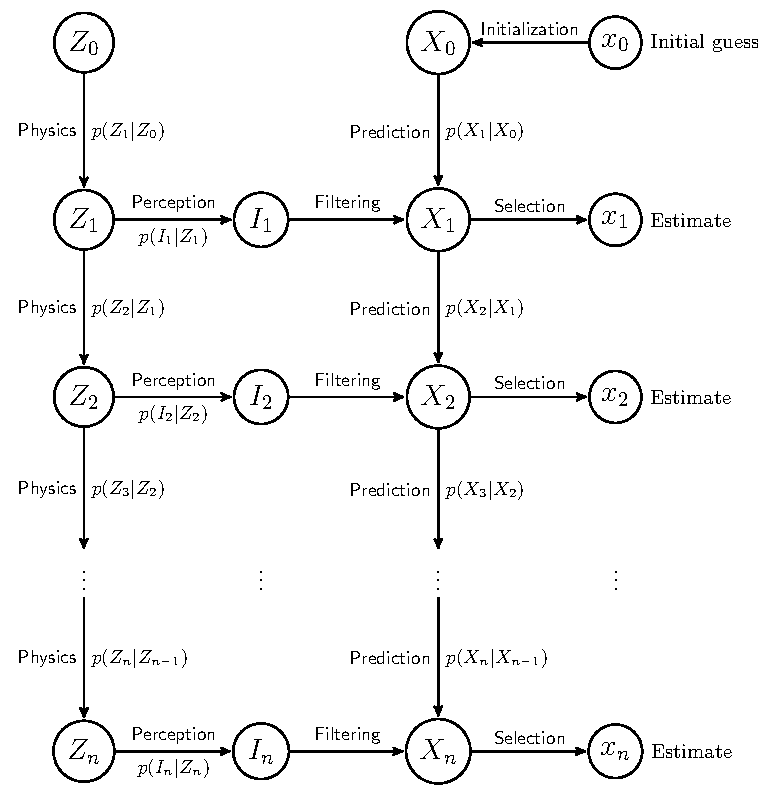
\includegraphics[width=0.2\textwidth]{figures/hmm-graph/hmm-graph.pdf}
An illustration of a Hidden Markov Model. The system assumes states $Z_1, Z_2, ...$ with probabilities $p(Z_1), p(Z_2|Z_1), \cdots$, and we obtain the observations $u_1, u_2, \cdots$ with probabilities $p(u_1|Z_1), p(u_2|Z_2), \cdots$.
